\chapter{Pointers in C++}

\section*{\Large \textbf{Pointers:}}
Pointers are variables that store the memory address of another variable. They are a powerful feature in C/C++ that allow direct memory access and manipulation. This chapter defines pointers, explains pointer-to-pointer, pointer arithmetic, and advanced pointer usage with examples, diagrams, and a comparison table.

\begin{figure}[h!]
  \centering
  \includegraphics[width=1\textwidth, height=10cm]{images/pointers.png}
  \caption{Pointer in C++}
  \label{fig:pointer_overview}
\end{figure}

\subsection*{\large \textbf{1. Definition and Explanation of Pointers}}

A \textbf{pointer} is a variable whose value is the address of another variable. For example, if we have an integer variable, its pointer will store the memory location where that integer is held.

\textbf{Key Points:}
\begin{itemize}[leftmargin=2em]
  \item Declaring a pointer: use the asterisk (\texttt{*}) before the pointer variable name.
  \item Dereferencing: the operator \texttt{*} is used to access the value at the memory address stored in the pointer.
  \item Address-of operator: the operator \texttt{\&} is used to get the memory address of a variable.
\end{itemize}

\subsection*{\large \textbf{2. Basic Pointer Usage in C++}}

\begin{lstlisting}[caption={Basic Pointer Example in C++}]
#include <iostream>
using namespace std;

int main() {
    int a = 42;
    int *ptr = &a;
    cout << "Value of a: " << a << endl;
    cout << "Address of a: " << &a << endl;
    cout << "Value stored in ptr (address of a): " << ptr << endl;
    cout << "Dereferenced ptr (value of a): " << *ptr << endl;
    return 0;
}
\end{lstlisting}

\subsection*{\large \textbf{3. Pointer to Pointer}}

A \textbf{pointer to pointer} stores the address of another pointer.

\begin{lstlisting}[caption={Pointer to Pointer in C++}]
#include <iostream>
using namespace std;

int main() {
    int a = 100;
    int *ptr = &a;
    int **pptr = &ptr;
    cout << "Value of a: " << a << endl;
    cout << "Address of a: " << &a << endl;
    cout << "ptr points to: " << ptr << endl;
    cout << "*ptr: " << *ptr << endl;
    cout << "pptr points to: " << pptr << endl;
    cout << "*pptr: " << *pptr << endl;
    cout << "**pptr: " << **pptr << endl;
    return 0;
}
\end{lstlisting}

\subsection*{\large \textbf{4. Pointer Arithmetic and Arrays}}

Pointer arithmetic is useful in array navigation. Adding 1 to a pointer makes it point to the next memory location of the pointed data type.

\begin{lstlisting}[caption={Pointer Arithmetic with Array in C++}]
#include <iostream>
using namespace std;

int main() {
    int arr[5] = {10, 20, 30, 40, 50};
    int *ptr = arr;
    cout << "Array elements using pointer arithmetic:" << endl;
    for (int i = 0; i < 5; i++) {
        cout << "Element " << i << ": " << *(ptr + i) << endl;
    }
    return 0;
}
\end{lstlisting}

\begin{figure}[H]
\centering
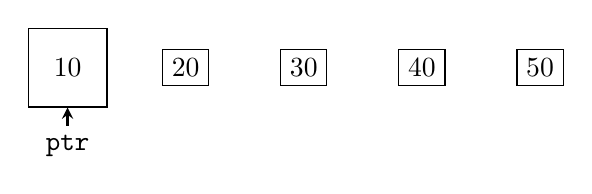
\begin{tikzpicture}[>=stealth, node distance=1.5cm]
    \node (a0) [draw, minimum width=1cm, minimum height=1cm] {10};
    \node (a1) [draw, right of=a0] {20};
    \node (a2) [draw, right of=a1] {30};
    \node (a3) [draw, right of=a2] {40};
    \node (a4) [draw, right of=a3] {50};

    \node (ptr) [below of=a0, yshift=0.5cm] {\texttt{ptr}};
    \draw[->, thick] (ptr.north) -- (a0.south);
\end{tikzpicture}
\caption{Pointer arithmetic: \texttt{ptr} points to \texttt{arr[0]}, \texttt{ptr+1} points to \texttt{arr[1]}, and so on.}
\end{figure}

\subsection*{\large \textbf{5. Table: Pointer Types and Use Cases}}

\begin{table}[H]
\centering
\begin{tabular}{|c|c|c|}
\hline
\textbf{Pointer Type} & \textbf{Declaration} & \textbf{Usage} \\
\hline
Single Pointer & \texttt{int *p;} & Holds address of an int \\
\hline
Double Pointer & \texttt{int **pp;} & Holds address of pointer to int \\
\hline
Null Pointer & \texttt{int *p = NULL;} & Indicates no address assigned \\
\hline
Void Pointer & \texttt{void *p;} & Generic pointer (typecast before use) \\
\hline
Function Pointer & \texttt{int (*fptr)(int);} & Points to a function \\
\hline
\end{tabular}
\caption{Common pointer types and their usage}
\end{table}

\section*{\Large \textbf{Summary}}
\begin{itemize}
  \item Pointers store memory addresses and enable dynamic memory access.
  \item They support arithmetic, point to arrays, and allow pointer-to-pointer usage.
  \item Advanced forms include void pointers, function pointers, and pointer arrays.
\end{itemize}